% Created by tikzDevice version 0.10.1 on 2018-01-12 16:14:57
% !TEX encoding = UTF-8 Unicode
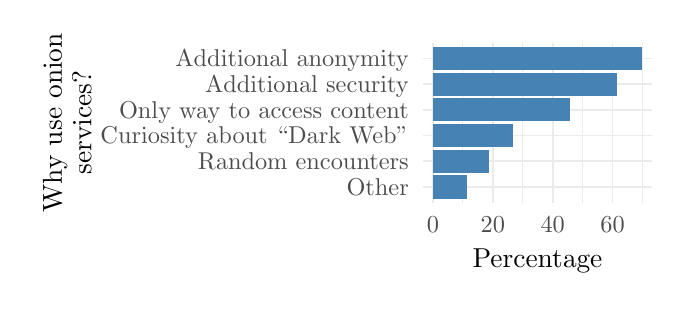
\begin{tikzpicture}[x=1pt,y=1pt]
\definecolor{fillColor}{RGB}{255,255,255}
\path[use as bounding box,fill=fillColor,fill opacity=0.00] (0,0) rectangle (231.26, 93.95);
\begin{scope}
\path[clip] (142.68, 30.77) rectangle (225.76, 88.45);
\definecolor{drawColor}{gray}{0.92}

\path[draw=drawColor,line width= 0.3pt,line join=round] (157.27, 30.77) --
	(157.27, 88.45);

\path[draw=drawColor,line width= 0.3pt,line join=round] (178.90, 30.77) --
	(178.90, 88.45);

\path[draw=drawColor,line width= 0.3pt,line join=round] (200.54, 30.77) --
	(200.54, 88.45);

\path[draw=drawColor,line width= 0.3pt,line join=round] (222.17, 30.77) --
	(222.17, 88.45);

\path[draw=drawColor,line width= 0.6pt,line join=round] (142.68, 36.35) --
	(225.76, 36.35);

\path[draw=drawColor,line width= 0.6pt,line join=round] (142.68, 45.66) --
	(225.76, 45.66);

\path[draw=drawColor,line width= 0.6pt,line join=round] (142.68, 54.96) --
	(225.76, 54.96);

\path[draw=drawColor,line width= 0.6pt,line join=round] (142.68, 64.26) --
	(225.76, 64.26);

\path[draw=drawColor,line width= 0.6pt,line join=round] (142.68, 73.57) --
	(225.76, 73.57);

\path[draw=drawColor,line width= 0.6pt,line join=round] (142.68, 82.87) --
	(225.76, 82.87);

\path[draw=drawColor,line width= 0.6pt,line join=round] (146.45, 30.77) --
	(146.45, 88.45);

\path[draw=drawColor,line width= 0.6pt,line join=round] (168.09, 30.77) --
	(168.09, 88.45);

\path[draw=drawColor,line width= 0.6pt,line join=round] (189.72, 30.77) --
	(189.72, 88.45);

\path[draw=drawColor,line width= 0.6pt,line join=round] (211.35, 30.77) --
	(211.35, 88.45);
\definecolor{fillColor}{RGB}{70,130,180}

\path[fill=fillColor] (146.45, 32.17) rectangle (158.77, 40.54);

\path[fill=fillColor] (146.45, 41.47) rectangle (166.57, 49.84);

\path[fill=fillColor] (146.45, 50.77) rectangle (175.40, 59.15);

\path[fill=fillColor] (146.45, 60.08) rectangle (196.12, 68.45);

\path[fill=fillColor] (146.45, 69.38) rectangle (212.96, 77.75);

\path[fill=fillColor] (146.45, 78.68) rectangle (221.99, 87.06);
\end{scope}
\begin{scope}
\path[clip] (  0.00,  0.00) rectangle (231.26, 93.95);
\definecolor{drawColor}{gray}{0.30}

\node[text=drawColor,anchor=base east,inner sep=0pt, outer sep=0pt, scale=  0.88] at (137.73, 33.32) {Other};

\node[text=drawColor,anchor=base east,inner sep=0pt, outer sep=0pt, scale=  0.88] at (137.73, 42.63) {Random encounters};

\node[text=drawColor,anchor=base east,inner sep=0pt, outer sep=0pt, scale=  0.88] at (137.73, 51.93) {Curiosity about ``Dark Web''};

\node[text=drawColor,anchor=base east,inner sep=0pt, outer sep=0pt, scale=  0.88] at (137.73, 61.23) {Only way to access content};

\node[text=drawColor,anchor=base east,inner sep=0pt, outer sep=0pt, scale=  0.88] at (137.73, 70.54) {Additional security};

\node[text=drawColor,anchor=base east,inner sep=0pt, outer sep=0pt, scale=  0.88] at (137.73, 79.84) {Additional anonymity};
\end{scope}
\begin{scope}
\path[clip] (  0.00,  0.00) rectangle (231.26, 93.95);
\definecolor{drawColor}{gray}{0.30}

\node[text=drawColor,anchor=base,inner sep=0pt, outer sep=0pt, scale=  0.88] at (146.45, 19.76) {0};

\node[text=drawColor,anchor=base,inner sep=0pt, outer sep=0pt, scale=  0.88] at (168.09, 19.76) {20};

\node[text=drawColor,anchor=base,inner sep=0pt, outer sep=0pt, scale=  0.88] at (189.72, 19.76) {40};

\node[text=drawColor,anchor=base,inner sep=0pt, outer sep=0pt, scale=  0.88] at (211.35, 19.76) {60};
\end{scope}
\begin{scope}
\path[clip] (  0.00,  0.00) rectangle (231.26, 93.95);
\definecolor{drawColor}{RGB}{0,0,0}

\node[text=drawColor,anchor=base,inner sep=0pt, outer sep=0pt, scale=  0.99] at (184.22,  7.44) {Percentage};
\end{scope}
\begin{scope}
\path[clip] (  0.00,  0.00) rectangle (231.26, 93.95);
\definecolor{drawColor}{RGB}{0,0,0}

\node[text=drawColor,rotate= 90.00,anchor=base,inner sep=0pt, outer sep=0pt, scale=  0.99] at ( 12.32, 59.61) {Why use onion};

\node[text=drawColor,rotate= 90.00,anchor=base,inner sep=0pt, outer sep=0pt, scale=  0.99] at ( 23.01, 59.61) {services?};
\end{scope}
\end{tikzpicture}
